\documentclass[10pt,a4paper]{article}

\usepackage[uft8]{inputenc}
\usepackage{graphicx}
\usepackage{enumerate}
%comentario
\title{Documento de prueba} %titulo del documento

\begin{document}
\section{Seccion que hablará de algo}
Hola.

Esto es un texto en \textbf{negrita}, \textit{cursiva} y \underline{subrayado}.

Desde este enlace entras a \href{www.google.com}{Google}.

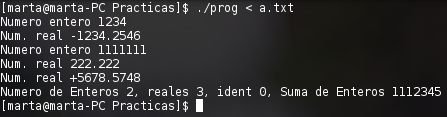
\includegraphics[width=0.7\textwidth]{1}

Vamos a listar cosas
\begin{itemize}
\item cosa 1
\item cosa 2
\item cosa 3
\end{itemize}

\begin{tabular}{l|l|l}
\hline
chocolate & chocolate & chocolate \\
pasteles & pasteles & pasteles \\
\end{tabular}

\end{document}